\documentclass{article}
\usepackage{aligned-overset}
\usepackage{amsmath}
\usepackage{amssymb}
\usepackage{bm}
\usepackage[shortlabels]{enumitem}
\usepackage{hyperref}
\usepackage[utf8]{inputenc}
\usepackage{mathtools}
\usepackage{physics}
\usepackage{tabularx}
\usepackage{titling}
\usepackage{fancyhdr}
\usepackage{xfrac}
\usepackage{pgfplots}

\definecolor{light-gray}{gray}{.9}

\pgfplotsset{compat = newest}

\author{Karsten Lehmann}
\date{SoSe 2021}
\title{Übung 02 Analysis - Weiterführende Konzepte}

\pagestyle{fancy}
\fancyhf{}
\lhead{\thetitle}
\rhead{\theauthor}
\lfoot{\thedate}
\rfoot{Seite \thepage}

\begin{document}

\section*{Existenz von Stammfunktionen}

Untersuchen Sie, ob folgenden Aussagen wahr oder falsch sind:

\begin{enumerate}[a)]
\item Jede Funktion $f \in R([a, b])$ besitzt auf $[a, b]$ eine Stammfunktion.

  \textit{Lsg.} Diese Aussage ist falsch.

  \textbf{Beweis mit Gegenbeispiel:}
  \begin{itemize}
  \item $f(x) = \frac{1}{x}, I = [a, b], 0 \notin I$.
    In diesem Fall ist $f$ stetig und beschränkt, somit ist
    $F(x) = \int_a^x f(t) \,dt$ die Stammfunktion $\Rightarrow$ das ist kein Gegenbeispiel
  \item $f = \begin{cases}
      0 & x = 0 \\
      \frac{1}{x} & x \ne 0 \\
    \end{cases}, I = [0, 1]$
    In diesem Fall ist $f$ nicht beschränkt, somit ist $f \notin R([0, 1])$
    $\Rightarrow$ das ist kein Gegenbeispiel
  \item $f = \begin{cases}
      1 & x \in [0, 1] \\
      -1 & x \in [-1, 0) \\
    \end{cases}, I = [-1, 1]$

    \begin{tikzpicture}
      \begin{axis}[
        axis lines=middle,
        xmax = 1.5,
        xmin = -1.5,
        ymax = 1.2,
        ymin = -1.2,]
        \addplot [
        domain=0:1,
        samples=100,
        very thick, blue]{1};
        \addplot [
        domain=-1:0,
        samples=100,
        very thick, blue]{-1};
      \end{axis}
    \end{tikzpicture}
  \end{itemize}

  $\Rightarrow f \in T([0, 1]) \subseteq R([0, 1])$

  $F(x) = \int_0^x f(t) \,dt = \begin{cases}
    x & x \in [0, 1] \\
    -x & x \in [-1, 0) \\
  \end{cases} = \abs{x}$

  $F$ ist auf $[-1, 1]$ nicht differenzierbar, da $f'(0)$ nicht existiert.

  $F_1(x) = x, x \in \underset{I_1}{\underbrace{[0, 1]}},
  F_2(x) = -x, x \in \underset{I_2}{\underbrace{[-1, 0]}}$.
  Dabei ist $F_1$ ist eine Stammfunktion auf $I_1$ und $F_2$ eine Stammfunktion
  auf $I_2$.
  Allerdings ist $F(x) = \begin{cases}
    F_1(x) & x \in I_1 \\
    F_2(x) & x \in I_2 \\
  \end{cases}$ keinen Stammfunktion auf $I_1 \cup I_2$.

  \fcolorbox{black}{light-gray}{
    \begin{minipage}{\textwidth}
      \textbf{Satz von Darboux} (Zwischenwertsatz für Ableitungen)
      
      Sei $I \in \mathbb{R}$ ein Intervall und $f \colon I \to \mathbb{R}$
      eine Differenzerbare Funktion, dann

      \[
        \forall c \in \left( \inf_{x \in I} f'(x) , \sup_{x \in I} f'(x) \right)
        \exists \eta \in I \colon f'(\eta) = c
      \]
    \end{minipage}
  }

  Aus dem Satz von Darboux folgt: Sprungfunktionen besitzen niemals Stammfunktionen.

  $\Rightarrow$ Funktionen mit einem Sprung, wie zum Beispiel $f(x) = sgn(x)$
  widerlegen die Aussage.

  
\item Ist $f$ auf $[a, b]$ differenzierbar, so ist $f'$ auf $[a, b]$ Riemann-integrierbar.

  \textit{Lsg.} Diese Aussage ist falsch.

  $f(x) = \begin{cases}
    x^2 \sin\left(\frac{1}{x^2}\right) & 0 < \abs{x} < 1 \\
    0 & x = 0 \\
  \end{cases}$

  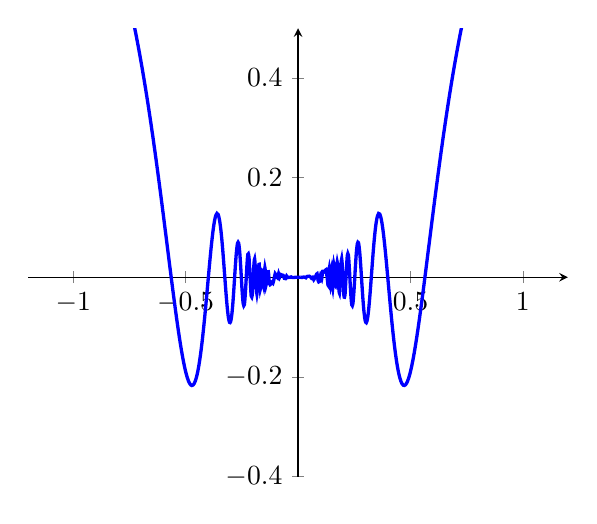
\begin{tikzpicture}
    \begin{axis}[
      axis lines=middle,
      xmax = 1.2,
      xmin = -1.2,
      ymax = 0.5,
      ymin = -0.4,]
      \addplot [
      domain=0.01:1,
      samples=200,
      smooth,
      very thick, blue]{x^2 * sin(deg(1 / x^2))};
      \addplot [
      domain=-1:0.01,
      samples=200,
      smooth,
      very thick, blue]{x^2 * sin(deg(1 / x^2))};
    \end{axis}
  \end{tikzpicture}

  
  \begin{align*}
    \Rightarrow x \ne 0 \colon f'(x) &= 2x \sin\left(\frac{1}{x^2}\right) + x^2 \cos\left(\frac{1}{x^2}\right)\left(-\frac{2}{x^3}\right) \\
                                     &= 2x \sin\left(\frac{1}{x^2}\right) - \colorbox{yellow}{$\frac{2}{x} \cos\left(\frac{1}{x^2}\right)$} \\
    x = 0 \colon f'(x) &= \lim_{h \to 0} \frac{f(h) - f(0)}{h} = \lim_{h \to 0} \frac{h^2 \sin\left(\frac{1}{h^2}\right)}{h} \\
                                     &= \lim_{h \to 0} h \cdot \underset{\abs{\ldots} \leq 1}{\underbrace{\sin\left(\frac{1}{h^2}\right)}} = 0 \\
  \end{align*}

  In der Ableitung ist ein \colorbox{yellow}{Ausdruck}, der dafür sorgt, dass diese nicht beschränkt ist.
  Sei $x_k = \frac{1}{\sqrt{2k\pi}} \in (0, 1]$

  \begin{align*}
    f'(x_k) &= \frac{2}{\sqrt{2k\pi}} \underset{= 0}{\underbrace{\sin(2k\pi)}} - 2 \sqrt{2k\pi} \underset{= 1}{\underbrace{\cos(2k\pi)}} \\
            &= - 2 \sqrt{2k\pi} \overset{k \to \infty}{\longrightarrow} -\infty
  \end{align*}
  
\end{enumerate}

\section*{Integration mittels Substitution}

Ermitteln Sie größtmögliche Intervalle $I \in \mathbb{R}$ auf denen die
folgenden Ausdrücke $f(x)$ Stammfunktionen besitzen.
Berechnen Sie zugehörige Stammfunktionen $F \colon I \to \mathbb{R}$
durch Anwendung des Hauptsatzes.


\textbf{Substitutionsregel}: $f(x) = g'(x) * h(g(x))$

$\Rightarrow F(x) = \int_{x_0}^x f(t) \,dt \overset{u = g(x)}= \int_{g(x_0)^{g(x)}} h(u) \,du$

Ist $H$ eine Stammfunktion von $h$ auf $[g(x), g(x_0)]$ (oder $[g(x_0), g(x)]$),
so folgt $F(x) = H(g(x)) - H(g(x_0))$
\begin{enumerate}[a)]
\item $f(x) = \frac{6}{1 - 3x}$

  $\mathbb{D}_f = \mathbb{R} \setminus \left\{ \frac{1}{3} \right\}$

  $\Rightarrow f$ besitzt jeweils auf den Intervallen
  $I_1 = \left( -\infty, \frac{1}{3} \right)$ und
  $I_2 = \left( \frac{1}{3}, +\infty \right)$ Stammfunktionen
  $F_1$ und $F_2$.

  $g(x) = 1 - 3x, g'(x) = -3 \Rightarrow f(x) = \frac{6}{g'(x)} \frac{g'(x)}{g(x)}
  = -2 \frac{g'(x)}{g(x)}$

  \begin{align*}
    x, x_k \in I_k, F_k(x) &= \int_{x_k}^x f(t) \,dt = -2 \cdot \int_{x_k}^x \frac{g'(x)}{g(x)} \,dt \\
                           &= \int_{x_k}^x \frac{6}{1 - 3t} \frac{-3}{-3} \,dt
                             \overset{h(u) = \frac{1}{u}}=  \\
                           &= _2 \int_{g(x_x)}^{g(x)} \frac{du}{u} = -2 \ln \abs{u} {\Big |}_{g(x_k)}^{g(x)}
                             = -2 \left( \ln \abs{g(x)} - \ln \abs{g(x_k)} \right) \\
                           &= -2 \ln \abs{\frac{g(x)}{g(x_k)}}
                             \underset{\underset{\substack{x, x_x \in I_k \Rightarrow \\  g(x), g(x_k) \text{ haben gleiches Vorzeicehn}}}\uparrow}=
    -2 \ln \frac{g(x)}{g(x_k)}
  \end{align*}

  $x_1 = 0, x_2 = \sfrac{2}{3} \Rightarrow F_k(x) = -2 \ln \abs{1 - 3x}, x \in I_k$

  \textbf{Achtung}: $\underset{\underset{\text{uneigentliches Riemann-Integral}}\Downarrow}{\int_{0}^{\sfrac{2}{3}} f(t) \,dt} \ne
  F_2\left(\sfrac{2}{3}\right) - F_1 (0)$ 
  
\item $f(x) = 3 \sqrt{8x - 4}$
\item $f(x) = \frac{1}{\sqrt[3]{5x - 7}}$
\item $f(x) = \frac{x}{4 + x^2}$

  $g(x) = 4 + x^2, g'(x) = 2x, f(x) = \frac{p(x)}{q(x)}, q$ besitzt keine reellen Nullstellen.

  \begin{align*}
    f(x) &= \frac{g'(x)}{2g(x)} \\
         &= \frac{1}{2} \int_0^x \frac{g'(t)}{2g(t)} \,dt \overset{h(u) = \sfrac{1}{u}}= \frac{1}{2} \int_{g(0)}^{g(x)} \frac{du}{u} \\
         &= \frac{\ln \abs{ub}}{2} {\Big |}_{\underset{> 0}{\underbrace{4}}}^{\underset{> 0}{\underbrace{4 + x^2}}} \\
         &= \frac{1}{2} \ln\left(\frac{4 + x^2}{4}\right), x \in \mathbb{R} \\
  \end{align*}
\item $f(x) = \frac{2x + 4}{x^2 + 4x + 7}$
\item $f(x) = \frac{x^2}{x^3 - 27}$
\item $f(x) = \frac{1}{x \cdot \ln x}$ 
\item $f(x) = 3e^x \sqrt{e^x + 1}$
\item $f(x) = \cos(x) \sin(2x)$

  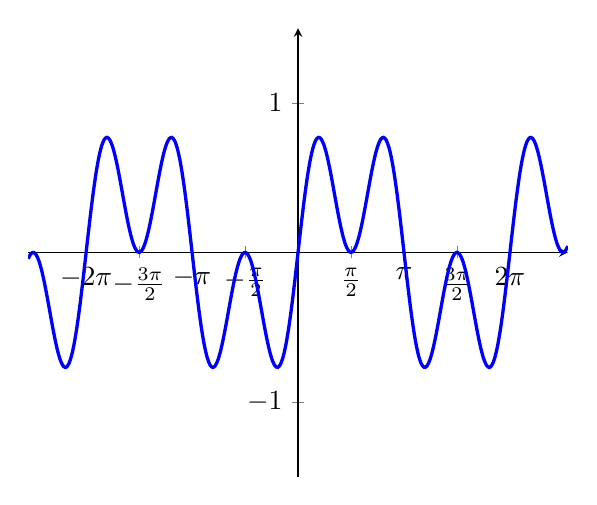
\begin{tikzpicture}
    \begin{axis}[
      axis lines=middle,
      xtick={-6.28318, -4.7123889, -3.14159, -1.5708, 1.5708, 3.14159, 4.7123889, 6.28318},
      xticklabels={$-2\pi$, $-\frac{3\pi}{2}$, $-\pi$ , $-\frac{\pi}{2}$, 
        $\frac{\pi}{2}$, $\pi$ , $\frac{3\pi}{2}$, $2\pi$},
      xmax = 8,
      xmin = -8,
      ymax = 1.5,
      ymin = -1.5,]
      \addplot [
      domain=-8:8,
      samples=200,
      smooth,
      very thick, blue]{cos(deg(x)) * sin(deg(2 * x))};
    \end{axis}
  \end{tikzpicture}
  
  $\mathbb{D}_f = \mathbb{R} \Rightarrow f$ ist auf jedem kompakten Intervall
  Riemann-integrierbar und $f$ besitzt auf $\mathbb{R}$ eine Stammfunktion.

  $F(x) = \int_0^x f(t) \,dt$ \textbf{Achtung} $f \notin R([-\infty, +\infty])$, da wir die
  Riemann-Integrale nur auf kompakten Intervallen erklärt haben.

  \fcolorbox{black}{light-gray}{
    \begin{minipage}{\textwidth}
      \textbf{Herleitung der Doppelwinkelformel}
      \begin{align*}
        e^{i(x + y)} &= e^{ix} \cdot e^{iy} = (\cos(x) + i\sin(x))(\cos(y) + i\sin(y)) \\
                     &= (\underset{\cos(x + y)}{\underbrace{\cos(x)\cos(y) - \sin(x)\sin(y)}}) +
                       i(\underset{\sin(x + y)}{\underbrace{\sin(x)\cos(y) + \cos(x)\sin(y)}}) \\
      \end{align*}
      Daraus folgt für $x = y \Rightarrow \substack{\cos(2x) = \cos^2(x) - \sin^2(x) \\ \sin(2x) = 2 \sin(x)\cos(x)}$
    \end{minipage}
  }
  
  \begin{align*}
    \text{Es gilt } f(x) &= \cos (x) \sin (2x) \overset{\text{Doppelwinkelformel}}= \cos (x) 2 \sin (x) \cos (x) \\
                         &= 2 \sin (x) \cos^2 (x) \\
  \end{align*}
  $g(x) = \cos(x), g'(x) = - \sin(x), h(u) = u^2 \Rightarrow f(x) = -2 g'(x) h(g(x))$

  \begin{align*}
    \Rightarrow F(x) &= \int_0^x f(t) \,dt = \int_{g(0)}^{g(x)} u^2 \,du = \frac{1}{3} u^3 {\Big |}_{g(0) = 1}^{g(x) = \cos(x)} \\
                     &= \frac{1}{3} (\cos^3 (x) - 1 ), x \in \mathbb{R} \\
  \end{align*}

   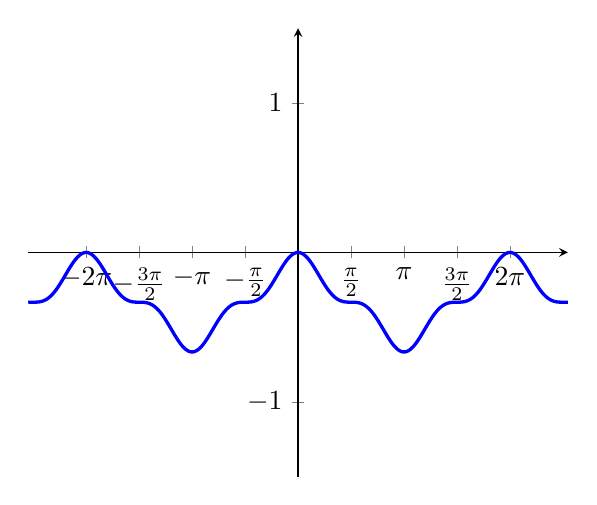
\begin{tikzpicture}
    \begin{axis}[
      axis lines=middle,
      xtick={-6.28318, -4.7123889, -3.14159, -1.5708, 1.5708, 3.14159, 4.7123889, 6.28318},
      xticklabels={$-2\pi$, $-\frac{3\pi}{2}$, $-\pi$ , $-\frac{\pi}{2}$, 
        $\frac{\pi}{2}$, $\pi$ , $\frac{3\pi}{2}$, $2\pi$},
      xmax = 8,
      xmin = -8,
      ymax = 1.5,
      ymin = -1.5,]
      \addplot [
      domain=-8:8,
      samples=200,
      smooth,
      very thick, blue]{1/3 * (cos(deg(x))^3 - 1)};
    \end{axis}
  \end{tikzpicture}
 \end{enumerate}

\section*{Integration mittels Substitution oder partieller Integration}

Ermitteln Sie größtmögliche Intervalle $I \in \mathbb{R}$ auf denen die
folgenden Ausdrücke $f(x)$ Stammfunktionen besitzen.
Berechnen Sie zugehörige Stammfunktionen $F \colon I \to \mathbb{R}$
durch Anwendung des Hauptsatzes.

\begin{enumerate}[a)]
\item $f(x) = x (\sin x^2 + \cos x^2)$
\item $f(x) = x^2 \sin x$
\item $f(x) = \exp\left( a \sqrt{x} + b \right), a \ne 0$
\item $f(x) = (x^2 -  4) \cos(2x)$
\item $f(x) = \frac{x^3 + 4x}{(x^2 + 4)^2}$
\item $f(x) = \exp(ax) \cos(bx), a, b \ne 0$
\end{enumerate}

\section*{Rekursionsformeln}

Stellen Sie für die folgenden Integrale
$F_n (x) \coloneqq \int_0^x f_n(t) \,dt, x \in \mathbb{R}$ und
$n \in \mathbb{N}_0$ Rekursionsformeln auf.
Geben Sie explizite Darstellungen von $F_0, \ldots, F_3$ an.

\fcolorbox{black}{light-gray}{
  \begin{minipage}{\textwidth}
    \textbf{Partielle Integration} $(u \cdot v)' = u'v + v'u$
    \begin{align*}
      \Rightarrow \int_{x_0}^x (u'v) \,dt &= \int_{x_0}^x (u \cdot v)' \,dt - \int_{x_0}^x v'u \,dt \\
                                          &= u \cdot v {\Big |}_{x_0}^x - \int_{x_0}^x v'u \,dt
    \end{align*}
  \end{minipage}
}
  

\begin{enumerate}[a)]
\item $f_n(t) = t^n e^{at}, a \ne 0$

  $f$ ist auf $\mathbb{R}$ stetig.

  $\Rightarrow \exists F_n(x) = \int_0^x f_n(t) \,dt$ für alle $x \in \mathbb{R}, n \in \mathbb{N}_0$

  \begin{align*}
    n = 0 &\colon F_0(x) = \int_0^x e^{at} \,dt = \frac{1}{a} e^{at} {\Big |}_{0}^x = \frac{1}{a} \left( e^{ax} - 1 \right), x \in \mathbb{R} \\
    n \geq 1 &\colon f_n(t) = t^n e^{at}, u(t) = t^n, v'(t) = e^{at} \Rightarrow u'(t) = n \cdot t^{n-1}, v(t) = \frac{1}{a} e^{at} \\
    \Rightarrow F_n(x) &= \int_0^x f_n(t) \,dt = \frac{t^n}{a} \cdot e^{at} {\Big |}_0^x - \int_0^x \frac{n}{a} t^{n-1} e^{at} \,dt \\
          &= \frac{x^n}{a} e^{ax} - \frac{n}{a} \underset{= F_{n - 1}(x)}{\underbrace{\int_0^x t^{n - 1} e^{at} \,dt}} \\
    \\
    F_1(x) &= \frac{x}{a} e^{ax} - \frac{1}{a} F_0(x) = \frac{x}{a} e^{ax} - \frac{1}{a^2} (e^{ax} - 1) \\
          &= \left( \frac{x}{a} - \frac{1}{a^2} \right) e^{ax} + \frac{1}{a^2} \\
    \\
    F_2(x) &= \frac{x^2}{a} e^{ax} - \frac{2}{a} F_1(x) = e^{ax} \left( \frac{x^2}{a} - \frac{x}{a^2} + \frac{1}{a^3} \right) - \frac{2}{a^3} \\
    \\
    F_3(x) &= \ldots
  \end{align*}
  
\item $f_n(t) = \sin^n(t)$

  $f$ ist auf $\mathbb{R}$ stetig.

  $\Rightarrow \exists F_n(x) = \int_0^x f_n(t) \,dt$ für alle $x \in \mathbb{R}, n \in \mathbb{N}_0$

  \begin{align*}
    n = 0 &\colon F_0(x) = \int_0^x 1 \,dt = x \\
    n = 1 &\colon F_1(x) = \int_0^x \sin(t) \,dt = \cos(x) {\Big |}_0^x = 1 - \cos{x} \\
    n \geq 2 &\colon u_n (t) = \sin^{n - 1} (t), v_n' = \sin (t) \\
          &\Rightarrow u_n' (t) = (n - 1) \sin^{n - 2}(t) \cos(t), v(t) = - \cos (t) \\
    \Rightarrow F_n(x) &= \int_0^x f(t) \,dt = - \cos(t) \cdot \sin^{n - 1} (t) {\Big |}_0^x - \int_0^x (n - 1) \sin^{n - 2}(t)\cos(t)(-\cos(t)) \,dt \\
          &= - \cos(x) \sin^{n - 1} (x) + (n - 1) \int_0^x \sin^{n - 2} (t) \underset{1 - \sin^2(t)}{\underbrace{\cos^2(t)}} \,dt \\
          &= - \cos(x) \sin^{n - 1} (x) + (n - 1) \int_0^x
            \underset{\sin^{n - 2} (t) - \sin^n(t)}{\underbrace{\sin^{n - 2} (t) \left(1 - \sin^2(t)\right)}} \,dt \\
          &= - \cos(x) \sin^{n - 1} (x) + (n - 1) F_{n - 2}(x) - F_n(x) \\
  \end{align*}
  \begin{align*}
    F_n(x) (1 + n - 1) = n F_n(x) &= - \cos(x) \sin^{n - 1}(x) + (n - 1) F_{n - 2}(x) \\
    F_n(x) &= \frac{1}{n} \cos(x) \sin^{n - 1} (x) + \frac{n - 1}{n} F_{n - 2}(x), x \in \mathbb{R} \\
    \\
    F_2(x) &= - \frac{1}{2} \cos(x) \sin(x) + \frac{1}{2}x \\
    \\
    F_3(x) &= - \frac{1}{3} \cos(x) \sin^2(x) + \frac{2}{3} (1 - \cos(x)) \\
  \end{align*}
\end{enumerate}

\section*{Stammfunktionen rationaler Funktionen}

Stammfunktionen von rationalen Funktionen können ermittelt werden, indem man den Polynomanteil abspaltet
und für den echt gebrochenen rationalen Restanteil eine \textit{Partialbruchzerlegung} der Form

\begin{align*}
  \frac{p(x)}{q(x)} &= \frac{p(x)}{(x - a)^k \cdot \ldots \cdot (x^2 + bx + c)^l \cdot \ldots} \\
                    &= \frac{A_1}{x - a} + \ldots + \frac{A_k}{(x - a)^k} + \ldots + \frac{B_1x + C_1}{x^2 + bx + c} + \ldots + \frac{B_lx + C_l}{(x^2 + bx + c)^l} + \ldots
\end{align*}

$(a, b, c, \ldots \in \mathbb{R}; k, l, \ldots \in \mathbb{N}$ ansetzt.
Die Ansatzkoeffizienten $A_1$, $\ldots$, $A_k$, $\ldots$,
$B_1$, $\ldots$, $B_l$, $\ldots$, $C_1$, $\ldots$, $C_l$, $\ldots$
lassen sich nach Multiplikation mit $g(x)$ durch \textit{Koeffizientenverschiebung} ermitteln.
Die entstehenden Partialbrüche führen auf Grundintegrale, die man kennen sollte.
Zu beachten sind hierbei die jeweiligen Existenzistervalle der Stammfunktionen, die
durch die Nullstellen des Nennerpolynoms vorgegeben sind.
Ermitteln Sie auf diesem Wege Stammfunktionen folgender Funktionen und zugehörige Existenzintervalle:

\begin{enumerate}[a)]
\item $f(x) \coloneqq \frac{2x^2 + 41x - 91}{(x + 3)(x - 1)(x - 4)}$

  $\mathbb{D}_f = \mathbb{R} \setminus \{ -3, 1, 4 \}$

  Stammfunktionen $F_k$ existieren auf den Intervallen $I_1 = (-\infty, -3)$, $I_2 = ( -3, 1 )$, $I_3 = ( 1, 4 )$,
  $I_4 = ( 4, +\infty )$

  \textbf{Partialbruchzerlegung}:
  \begin{align*}
    f(x) = \frac{p(x)}{q(x)} &= \frac{A}{x + 3} + \frac{B}{x - 1} + \frac{C}{x - 4} \\
                             &= \frac{A(x - 1)(x - 4) + B(x + 3)(x - 4) + C(x + 3)(x - 1)}{q(x)} \\
  \end{align*}

  $\Rightarrow A(x - 1)(x - 4) + B(x + 3)(x - 4) + C(x + 3)(x - 1) = p(x) = 2x^2 + 41x - 91$

  Bestimmung von $A, B, C$ durch Einsetzen der Nullstellen:
  \begin{align*}
    x = -3 &\colon A(-4)(-7) = 28A = 2 (-3)^2 + 41 (-3) - 91 = -196 \Rightarrow A = -7 \\
    x = 1 &\colon B(4)(-3) = -12B = 2 \cdot 1^2 + 41 \cdot 1 - 91 = -48 \Rightarrow B = 4 \\
    x = 4 &\colon C(7)(3) = 21C = 2 \cdot 4^2 + 41 \cdot 4 - 91 = 105 \Rightarrow C = 5 \\
  \end{align*}

  \begin{align*}
    x, x_x \in I_k &\colon F_k(x) = \int_{x_k}^x - \frac{7}{t + 3} + \frac{4}{t - 1} + \frac{5}{t - 4} \, dt \\
                   &= \left( -7 \ln\abs{t + 3} + 4 \ln\abs{t - 1} + 5 \ln\abs{t - 4} \right) {\Big |}_{x_k}^x
  \end{align*}
\item $f(x) \coloneqq \frac{x + 2}{x^3 - 2x^2 + x}$
\item $f(x) \coloneqq \frac{x^2 + 11x - 1}{(x^2 + 1)(x - 2)}$
\end{enumerate}

\end{document}